\documentclass[12pt]{article}

% Packages
\usepackage{amsmath}
\usepackage{amsthm}
\usepackage{graphicx}
\usepackage{hyperref}
\usepackage{geometry}
\usepackage{fancyhdr}
\usepackage{cite}
\usepackage{algorithm}
\usepackage{algorithmic}
\usepackage{pgfplots}
\pgfplotsset{compat=1.18}

% Page layout
\geometry{a4paper, margin=1in}

% Header and Footer
\pagestyle{fancy}
\fancyhf{}
\fancyhead[L]{X.B. Wang, Y.Y. Lu}
\fancyhead[C]{Survey on Randomized Algorithms on Graphs}
\fancyhead[R]{\thepage}

% Title
\title{Survey on Randomized Algorithms on Graphs}
\author{
    Wang Xianbang\thanks{Email: \texttt{wang-xb24@mails.tsinghua.edu.cn}} \\
    IIIS, Tsinghua University
    \and
    Lu Yiyang\thanks{Email: \texttt{WOBUZHIDAO@mails.tsinghua.edu.cn}} \\
    IIIS, Tsinghua University
}
\date{\today}

\newtheorem{lemma}{Lemma}

\begin{document}

\maketitle

% Abstract
\begin{abstract}
    Sheng Si Ju Ji Xue Bing Wang, Jian Xian Si Qi Fu Tou Bang.
\end{abstract}

% Introduction
\section{APSP: All Pairs Shortest Path}
\subsection{Introduction}

One of the well-known result in randomized algorithms in graph theory is the algorithm for the \textbf{All Pairs Shortest Path (APSP)} problem.

Let $G(V,E)$ be an \textbf{undirected} graph, with $V=\{1,2,\cdots,n\}$ and $|E|=m$. Let the adjacency matrix of $G$ be $A$, where $A_{ij}=A_{ji}=1$ if $(i,j)\in E$ and $A_{ij}=A_{ji}=0$ otherwise. There is a weak version of the APSP problem, \textbf{All Pairs Distance (APD)} problem, which is to compute the distance between all pairs of vertices in $G$, i.e., derive the \emph{distance matrix} $D$ where $D_{ij}$ is the length of the shortest path between $i$ and $j$.

The requirement of APSP is stronger: it requires the algorithm to compute the shortest path itself, not just the length of the shortest path, of all pairs of vertices in $G$. 

If $G$ is not connected, we can seperate $G$ into connected components and solve the APSP problem for each connected component (finding connected components is easy and can be done in linear time). So we assume $G$ is \textbf{connected} in the following discussion.

Note that, if we want to store all the shortest paths, the space complexity can be $\Omega(n^3)$ (e.g. a path), which limits the time complexity we can achieve. However, we can record an \emph{implicit} representation of the shortest path - the \textbf{successor matrix} $S$: for every $(u,v)\in V^2$, let $S_{uv}$ be the vertex that is the immediate successor of $u$ on the shortest path from $u$ to $v$. This can be stored in $O(n^2)$ space, and the shortest path from $u$ to $v$ can be reconstructed by following the path $u\to S_{uv}\to S_{S_{uv}v}\to\cdots\to v$ in $O(L)$ time, where $L$ is the length of the shortest path.

\subsection{Quick Review on Deterministic Algorithms}

The most well-known algorithm for APSP is the \textbf{Floyd-Warshall} algorithm, which has a time complexity of $O(n^3)$. The algorithm is based on dynamic programming, and the key idea is to consider all vertices as potential intermediate vertices in the shortest path. The algorithm is simple and easy to implement.

Another algorithm is based on \textbf{breadth-first search (BFS)}: for every vertex $v$, run a BFS starting from $v$ to compute the shortest path from $v$ to all other vertices. This algorithm has a time complexity of $O(nm)$, which is better when $m=o(n^2)$.

For weighted graph (every edge has a weight), the \textbf{Johnson} algorithm can be used to solve the APSP problem. The time complexity can achieve $O(nm+n^2\log n)$ using Fibonacci heap. This algorithm is an extension of Dijkstra's algorithm, which is only applicable in non-negative weight circumstance. 

It is clear that the best time complexity we can achieve for APSP is $\Omega(n^2)$, since we need to output $n^2$ shortest paths. And we also believe that $O(nm)$ is still far away from the best, especially if $m=\Omega(n^2)$.

\subsection{Matrix Multiplication-based Algorithm}

Now we introduce a randomized algorithm for APSP, which is based on matrix multiplication. The algorithm is proposed by Alon, Galil, and Margalit in 1994.

\subsubsection{Skim on Matrix Multiplication}

Given two $n\times n$ matrices $A$ and $B$, the product $C=AB$ is defined as $C_{ij}=\sum_{k=1}^n A_{ik}B_{kj}$. The naive algorithm has a time complexity of $O(n^3)$. The lower bound of matrix multiplication is obviously $\Omega(n^2)$, and computer scientists have been trying to find a better exponent $2<\alpha<3$ until now.

Strassen proposed a divide-and-conquer algorithm in 1969, which has a time complexity of $O(n^{\log_2 7})\approx O(n^{2.81})$. According to Wikipedia, as of January 2024, the best peer-reviewed matrix multiplication algorithm is by Virginia Vassilevska Williams, Yinzhan Xu, Zixuan Xu, and Renfei Zhou and has complexity $O(n^{2.371552})$. It is still an open problem to find a matrix multiplication algorithm with complexity $O(n^{2+o(1)})$, or prove that such an algorithm does not exist.

\emph{From now on, suppose we have a matrix multiplication algorithm with time complexity $O(n^\nu)$.}

\subsubsection{APD}
Recall that $A$ is adjacent matrix. Let $\bar{A}$ be the matrix where $\bar{A}_{ij}=1$ if $i=j$ or $A_{ij}=1$. The connection between shortest path and matrix multiplication is revealed by the following lemma.
\begin{lemma}
    \label{lemma:shortest_path_matrix_multiplication}
    Let $k$ be an positive integer. For every $i,j\in V$, $D_{ij}\le k$ if and only if $\bar{A}^k_{ij}>0$.
\end{lemma}
\begin{proof}
If $\bar{A}^k_{ij}>0$, considering the procedure of matrix multiplication, there must be $i_0=i,i_1,i_2,\cdots,i_k=j\in V$, such that $\bar A_{i_0i_1}=\bar A_{i_1i_2}=\cdots=\bar A_{i_{k-1}i_k}=1$. So there is a path $i_0\to i_1\to i_2\to\cdots\to i_k$ of length $k$ from $i$ to $j$, which implies $D_{ij}\le k$.
\end{proof}

The lemma implies that we can compute the distance matrix $D$ by computing $\bar{A}^k$ for $k=1,2,\cdots,n$. However, this requires $O(n^{\nu+1})=\omega(n^3)$ time, which is even worse.

The idea to improve this is: we compute $\bar A^2$, which can reduce the length of the shortest path to a half, and do the computation recursively. We should first get $A'$, where $A'_{ij}=1$ if $A_{ij}=1$ or there is a path of length 2 from $i$ to $j$. From Lemma \ref{lemma:shortest_path_matrix_multiplication}, we can derive $A'$ from $\bar A^2$ in $O(n^2)$: $A'_{ij}=1$ iff $\bar A_{ij}>0$.

Recursively run the algorithm on $A'$ (which also represents a graph $G'$), and suppose we got a distance matrix $D'$ for $G'$. Now we want to retrieve $D$.

\begin{lemma}
\label{2}
For every $i,j\in V$, $D'_{ij}=\lceil\dfrac{D_{ij}}{2}\rceil$.
\end{lemma}
\begin{proof}
Due to the definition of $A'$, $D'$ represents the distance, where we can walk 2 steps at a time. The lemma is then obvious.
\end{proof}

Lemma \ref{2} is inadequate because given $D'$, every element of $D$ has two choices. However, Lemma \ref{3} could tell us the answer.
\begin{lemma}
\label{3}
Let $i\not=j \in V$. For any neighbor $u$ of $i$ in $G'$, $D_{ij}-1\le D_{uj}\le D_{ij}+1$. And there exists at least one $u$, such that $D_{uj}=D_{ij}-1$.
\end{lemma}
\begin{proof}
For any neighbor $u$, we can first go to $i$, and walk $D_{ij}$ steps to $j$. Thus, there is a path from $u$ to $j$ of length $D_{ij}+1$, implying $D_{uj}\le D_{ij}+1$. Interchange $i$ and $u$, we can get $D_{uj}\ge D_{ij}-1$. Suppose the shortest path between $i,j$ is $i\to i_1\to\cdots\to i_t=j$, then $D_{i_1j}=D_{ij}-1$.
\end{proof}

\begin{lemma}
\label{4}
If $D_{ij}$ is even, $D'_{kj}\ge D'_{ij}$ for every neighbor $k$ of $i$; if $D_{ij}$ is odd, $D'_{kj}\le D'_{ij}$ for every neighbor $k$ of $i$, and at least one equality does not hold.
\end{lemma}
\begin{proof}
Suppose $D_{ij}=2t$ is even. Lemma \ref{3} tells $D_{kj}\in\{2t-1,2t,2t+1\}$ for every neighbor $k$ of $i$. Use Lemma \ref{2}, $D'_{kj}\ge t=D'_{ij}$. \\
Now suppose $D_{ij}=2t+1$ is odd, then $D_{kj}=\{2t,2t+1,2t+2\}$, so $D'_{kj}\in \{t,t+1\}$, thereby $\le t+1=D'_{ij}$. And at least one $k$ satisfies $D_{kj}=D_{ij}-1=2t$, so $D'_{kj}=t<D'_{ij}$.
\end{proof}

In fact, to compute $D$ from $D'$, we only need to know the parity of each $D_{ij}$. From Lemma \ref{4}, we can seperate even and odd $D_{ij}$, and compute $D$ in $O(n^2)$ time. Specifically, $D_{ij}$ is even iff
$$\sum\limits_{k\text{ is neighbor of }i} D'_{kj}\ge d_iD_{ij},$$
$d_i$ is the degree of $i$. If $S=AD'$, then $D_{ij}$ is even iff $S_{ij}\ge d_iD_{ij}=\bar A^2_{ii}D_{ij}$. The implementation is shown in Algorithm \ref{alg:example}.

\begin{algorithm}
\caption{APD}
\label{alg:example}
\begin{algorithmic}
    \STATE \textbf{Input:} Graph $G=(V,E)$ with adjacency matrix $A$
    \STATE \textbf{Output:} Distance matrix $D$
    \STATE $\bar A\leftarrow I+A$
    \STATE $A^*\leftarrow \bar A^2$
    \FOR{$i=1$ to $n$}
        \FOR{$j=1$ to $n$}
            \STATE $A'_{ij}\leftarrow 1$ if $A_{ij}=1$ or ${A^*}_{ij}>0$
        \ENDFOR
    \ENDFOR
    \STATE $D'\leftarrow$ APD$(A')$
    \STATE $S\leftarrow AD'$
    \FOR{$i=1$ to $n$}
        \FOR{$j=1$ to $n$}
            \STATE $D_{ij}\leftarrow 2D'_{ij}$ if $S_{ij}\ge A^*_{ii}D'_{ij}$, otherwise $D_{ij}\leftarrow 2D'_{ij}-1$
        \ENDFOR
    \ENDFOR
    \RETURN $D$
\end{algorithmic}
\end{algorithm}

\subsubsection{APSP}

Observe that, the preceding algorithm does not provide enough information of successor matrix $S$. More precisely, if $D_{ij}$ is even, it is not guaranteed from Lemma \ref{4} that we can find $k$ just from $D'$.

Suppose $D$ is computed with algorithm \ref{alg:example}. For every $i,j\in V$, how to find $S_{ij}$? Or, what is the necessary and sufficient condition of $S_{ij}$? The answer of the last question is clear: $(i,S_{ij})\in E$, and $D_{ij}-1 = D_{S_{ij}j}$. Let $r=D_{ij}$. For every integer $u\ge 0$, define $D^{(u)}$ as: $D^{(u)}_{ij}=1$ iff $D_{ij}=u$. So $S_{ij}$ is one of the \textbf{witness} of $A$ and $D^{(r-1)}$ w.r.t $i,j$. (\emph{Note: the witness of two matrices $A$ and $B$ w.r.t. $i,j$ is an index $x$ that $A_{ix}=B_{xj}=1$.})

Given two 0-1 matrices $A,B$, to compute a \textbf{witness matrix} is a well-known problem in computer science called \textbf{Boolean Product Witness Matrix (BPWM)}. We will leave the implementation of BPWM in section \ref{sec:bpwm}.

\subsubsection{BPWM}
\label{sec:bpwm}

\subsubsection{Small Improvement}

\subsection{Experimental Results}

We implemented four algorithms for APSP: for the deterministic algorithms, we implemented Floyd-Warshall and BFS; for the randomized algorithms, we implemented the matrix multiplication-based algorithm with two versions: one with Strassen's algorithm and the other with the trivial matrix multiplication.

Algorithms are implemented with C++.

\subsubsection{Settings}

We set the graph size to be $n=2^k$, where $k\le 8$. In our experiment, edges are independently and uniformly generated, each with probability $p$. To ensure the graph is connected, after graph is randomly generated, we add $M-1$ edges to connect the graph, where $M$ is the number of connected components.

Our test environment is $\texttt{-std=C++11}$ and has unlimited stack size. 

\subsubsection{Parameters}

We set $\gamma=3$ in BPWM, and the threshold of Strassen's algorithm to be $n_0=64$. $p=0.1$ since we do not want the graph to be too dense, and also limit the performance of BFS.

\subsubsection{Results}

We run the algorithms for 5 times and record the average execution time. The results of $k=7,8$ ($n=128,256$) are shown in Figure \ref{fig:et}. 

An interesting phenomenon is, when $k$ increase by 1, the execution time of \texttt{BFS} and \texttt{Floyd} increase by a factor of $3\sim 4$, while the execution time of \texttt{Strassen} and \texttt{Trivial} increase by a factor of $5\sim 6$. This is partially due to the optimization of C++ compiler, which can optimize the loops in \texttt{BFS} and \texttt{Floyd} to be more cache-friendly - but not the case when there are heavy matrix multiplications.

\begin{figure}[h]
    \centering
    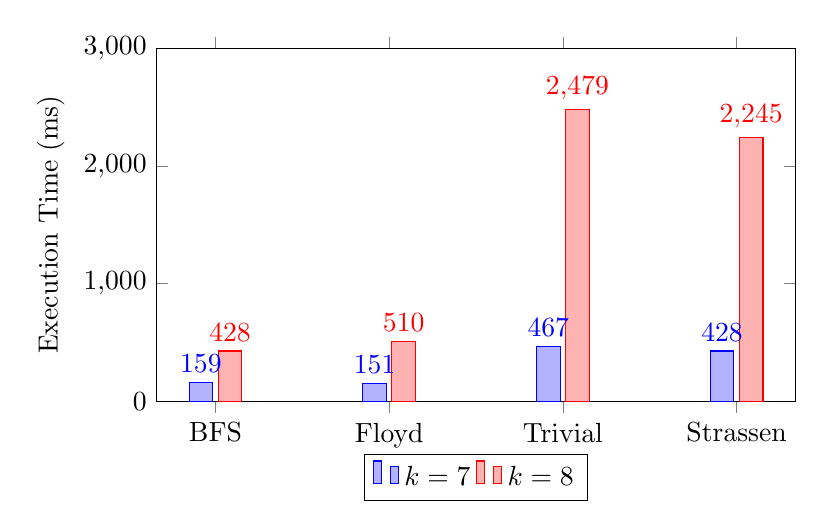
\begin{tikzpicture}
        \begin{axis}[
            ybar,
            bar width=0.3cm,
            width=0.8\textwidth,
            height=0.5\textwidth,
            symbolic x coords={BFS, Floyd, Trivial, Strassen},
            xtick=data,
            ylabel={Execution Time (ms)},
            xlabel={Algorithms},
            ymin=0,
            ymax=3000,
            legend style={at={(0.5,-0.15)}, anchor=north, legend columns=-1},
            nodes near coords,
            enlarge x limits={abs=0.75cm}
        ]
        \addplot coordinates {(BFS, 159) (Floyd, 151) (Trivial, 467) (Strassen, 428)};
        \addplot coordinates {(BFS, 428) (Floyd, 510) (Trivial, 2479) (Strassen, 2245)};
        \legend{$k=7$, $k=8$}
        \end{axis}
    \end{tikzpicture}
    \caption{Execution time of different algorithms on two datasets}
    \label{fig:et}
\end{figure}

\subsubsection{Analysis}

Granted, although the time complexity of \texttt{Strassen} is better than \texttt{BFS} and \texttt{Floyd}, the actual execution time is much larger. This is because the constant factor of Strassen's algorithm is remarkably large. Moreover, if the parameter is not carefully chosen, or $p$ is much smaller, \texttt{BFS} will perform even better and \texttt{Strassen} and \texttt{Trivial} will be even worse. Consequently, the matrix multiplication-based algorithm has less practical significance than theoretical significance.

Based on the data of $k=8$, we can approximate the constant factor of these algorithms. Suppose the execution time of \texttt{Floyd} is $\beta\cdot n^3$, and the execution time of \texttt{Strassen} is $\alpha\cdot n^{\log_2 7}\log n$. Plugging in the data, we can get $\alpha\approx 3.9\cdot 10^{-4}$ and $\beta\approx 8.5\cdot 10^{-5}$. Finding the threshold $N$, which satisfies $\alpha\cdot N^{\log_2 7}\log N=\beta\cdot N^3$, we can get $N\approx 2500$. 

Since for $n=2^k$, Strassen's algorithm is much faster than other cases (which need to expand the matrix up to $4$ times of parameters), we can extrapolate that the actual threshold should be $N_0\approx 10^4$. \texttt{Strassen} will likely be faster than \texttt{Floyd} when $n\gg N_0$; if we replace Strassen's matrix multiplication with the most advanced algorithm, we surmise that the threshold will be slightly lower.

\subsection{Extensions}

\subsubsection{Derandomization}
\subsubsection{Directed Graph}
\subsubsection{Weighted Graph}

\subsection{Open Problems}

\end{document}